\documentclass[aspectratio=169,10pt]{beamer}
\usepackage{bookmark}
\usepackage{pifont}
\usepackage{booktabs}
\usepackage{tikz}
\usepackage{adjustbox}
\usepackage{float}
\usepackage{longtable}
\usepackage{amsfonts}
\usepackage{csquotes}
\usepackage{ragged2e}
\usepackage{color, colortbl}
\usepackage[spanish,mexico]{babel}
\usepackage[spanish]{algorithm2e}
\usepackage{media9}
\usepackage{multirow}
\usepackage{booktabs}
\usepackage{hyperref}
\usepackage[style=apa]{biblatex}
\usepackage[caption=false]{subfig}
% \usepackage[duration=20,lastminutes=5]{pdfpcnotes}
\usepackage{pgfpages}
% \setbeameroption{show notes on second screen=right}

\title{Deep Learning aplicado a la salud}
\subtitle{Detección de cáncer en imágenes citológicas}
\author[M.I.I Marco del Moral]{Marco Julio del Moral Argumedo}
\institute[ITO]{Tecnológico Nacional de México/Instituto Tecnológico de Orizaba}
\date{18 de mayo de 2022}

\definecolor{LightCyan}{rgb}{0.88,1,1}
\definecolor{titlepagecolor}{cmyk}{1,.60,0,.40}
\definecolor{namecolor}{cmyk}{1,.50,0,.10}
\definecolor{portadaa}{RGB}{73, 86, 120}
\definecolor{azul}{rgb}{0.768, 0.729, 0.949}
\definecolor{verde}{rgb}{0.847, 0.949, 0.729}
\definecolor{media}{rgb}{0.909, 0.670, 0.886}
\newcommand\insertlogoii{}
\newcommand\logoii[1]{\renewcommand\insertlogoii{#1}}
\special{pdf:minorversion 7}
\usetheme[]{Berkeley}    % JuanLesPins Berkeley PaloAlto Warsaw Goettingen Marburg
\usefonttheme{default} % default professionalfonts serif structurebold structureitalicserif structuresmallcapsserif
\usecolortheme{albatross} % albatross beaver beetle crane dolphin fly lily orchid rose seahorse seagull whale default
\useinnertheme{rectangles}
\setbeamerfont{section in sidebar}{size=\fontsize{5}{6}\selectfont}
\setbeamerfont{subsection in sidebar}{size=\fontsize{4}{5}\selectfont}
\setbeamerfont{subsubsection in sidebar}{size=\fontsize{3}{4}\selectfont}
\makeatletter

\setbeamertemplate{footline}
        {
      \leavevmode%
      \hbox{%
      \begin{beamercolorbox}[wd=.333333\paperwidth,ht=2.2ex,dp=1ex,center]{author in head/foot}%
        \usebeamerfont{author in head/foot}marcojulioarg@gmail.com
      \end{beamercolorbox}%
      \begin{beamercolorbox}[wd=.333333\paperwidth,ht=2.2ex,dp=1ex,center]{title in head/foot}%
        \usebeamerfont{title in head/foot}\insertshorttitle
      \end{beamercolorbox}%
      \begin{beamercolorbox}[wd=.333333\paperwidth,ht=2.2ex,dp=1ex,center]{date in head/foot}%
        \usebeamerfont{date in head/foot}\insertframenumber\,/\,\inserttotalframenumber%\hspace*{2em}

    %#turning the next line into a comment, erases the frame numbers
        %\insertframenumber{} / \inserttotalframenumber\hspace*{2ex}

      \end{beamercolorbox}}%
      \vskip0pt%
    }

\setbeamertemplate{headline}
    {%
      \begin{beamercolorbox}[wd=\paperwidth]{frametitle}
        \ifx\beamer@sidebarside\beamer@lefttext%
        \else%
          \hfill%
        \fi%
        \ifdim\beamer@sidebarwidth>0pt%
          \usebeamercolor[bg]{logo}%
          \vrule width\beamer@sidebarwidth height \beamer@headheight%
          \hskip-\beamer@sidebarwidth%
          \hbox to \beamer@sidebarwidth{\hss\vbox to
            \beamer@headheight{\vss\hbox{\color{fg}\insertlogo}\vss}\hss}%
          \hfill%
          \vrule width\beamer@sidebarwidth height \beamer@headheight%
          \hskip-\beamer@sidebarwidth%
          \hbox to \beamer@sidebarwidth{\hss\vbox to
            \beamer@headheight{\vss\hbox{\color{fg}\insertlogoii}\vss}\hss}%
        \else%
          \vrule width0pt height \beamer@headheight%
        \fi%
      \end{beamercolorbox}
  }
  \makeatother
  \makeatletter
    \setbeamertemplate{sidebar \beamer@sidebarside}%{sidebar theme}
    {
      \beamer@tempdim=\beamer@sidebarwidth%
      \advance\beamer@tempdim by -6pt%
      \insertverticalnavigation{\beamer@sidebarwidth}%
      \vfill
      \ifx\beamer@sidebarside\beamer@lefttext%
      \else%
        \usebeamercolor{normal text}%
        \llap{\usebeamertemplate***{navigation symbols}\hskip0.1cm}%
        \vskip2pt%
      \fi%
  }%
  \makeatother

\graphicspath{ {imagenes/} }

\logo{
\includegraphics[height=1cm]{logo_transparente}}
\logoii{
\includegraphics[height=1cm]{CONACYT1-2}}


\begin{document}

\begin{frame}
  \titlepage
\end{frame}

\section{Introducción}

\begin{frame}{Introducción}{Reseña del curso}
  El curso se desarrolló para mostrar como se usa el Deep Learning, en particular, aplicado a la salud.
  \begin{exampleblock}{Objetivos}
    \begin{enumerate}
      \item Aprender nociones básicas de lenguaje Python aplicado.
      \item Analizar las técnicas algorítmicas de aprendizaje computacional.
      \item Entender el funcionamiento básico de modelos populares.
      \item Conocer la metodología de evaluación para un modelo de clasificación.
      \item Entrenar modelos para encontrar soluciones al problema expresado.
    \end{enumerate}
  \end{exampleblock}
\end{frame}

\section{Definición del problema}

\subsection{Aplicaciones de I.A. en salud}

\begin{frame}{Aplicaciones}{Chatbots}
  Un chatbot es una herramienta basada en Procesamiento de Lenguaje Natural que permite a una persona establecer comunicación directa con un sistema inteligente.
  \begin{figure}[]
    \centering
    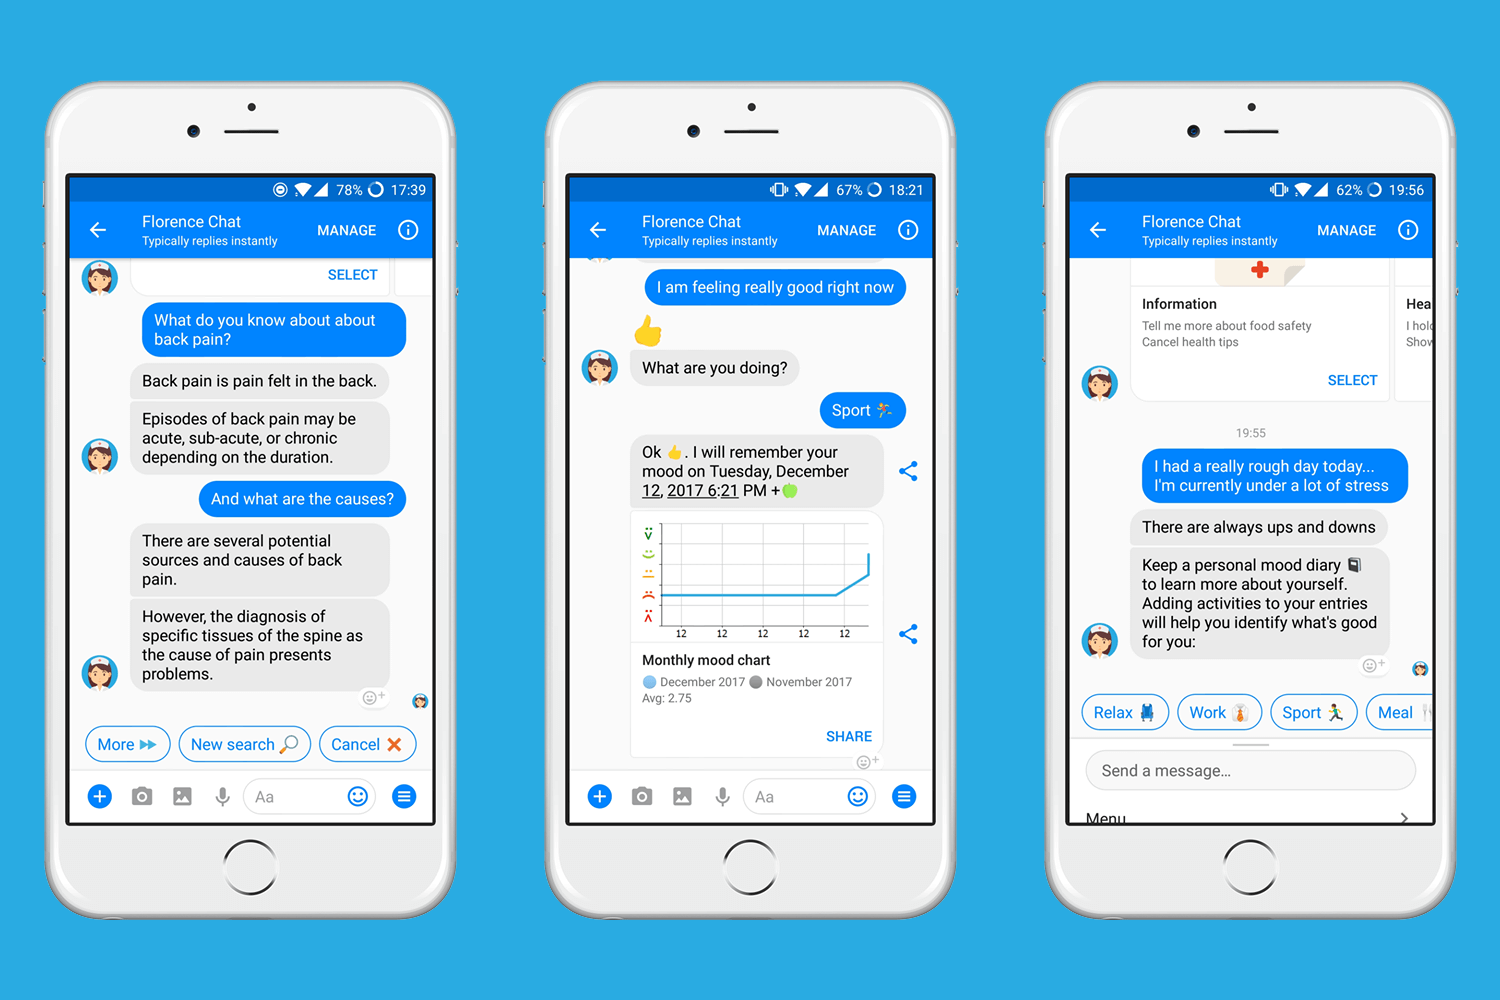
\includegraphics[height=0.8\textheight]{chatbot}
  \end{figure}
\end{frame}

\begin{frame}{Aplicaciones}{Cirugías robóticas}
  La cirugía robótica asistida por I.A. permite a los robots llevar a cabo cirugías de manera automatizada con mínima supervisión.
  \begin{figure}[]
    \centering
    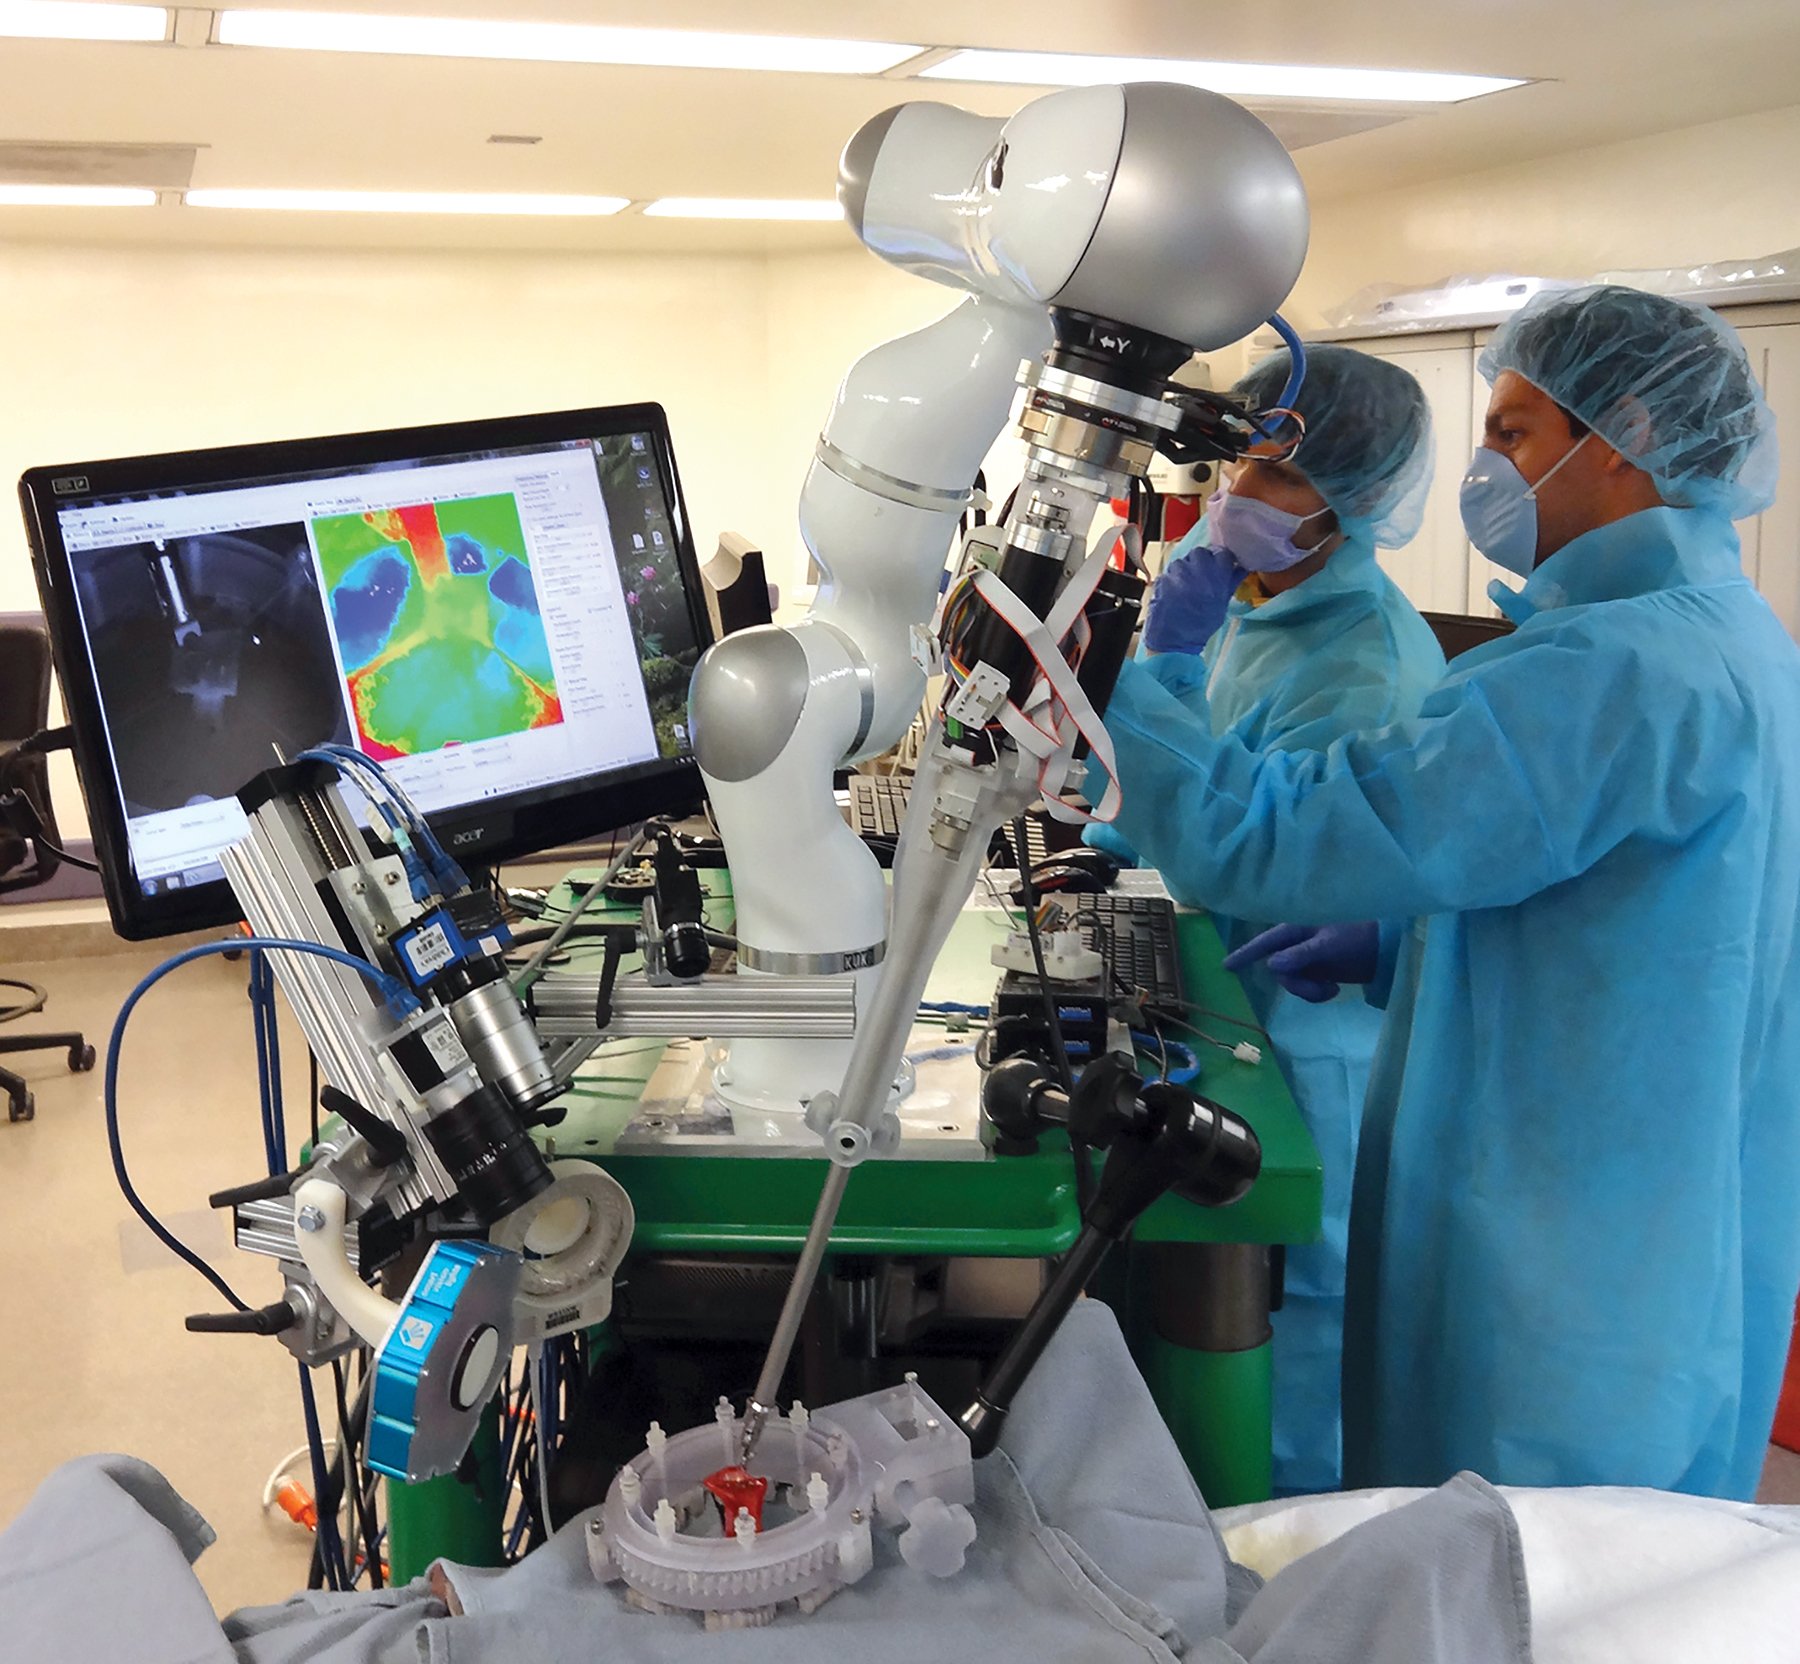
\includegraphics[height=0.8\textheight]{cirugia.jpg}
  \end{figure}
\end{frame}

\begin{frame}{Aplicaciones}{Descubrimiento de medicinas}
  La I.A. es capaz de encontrar nuevas fórmulas para medicinas analizando grandes volúmenes de datos y creando conocimiento por si mismas.
  \begin{figure}[]
    \centering
    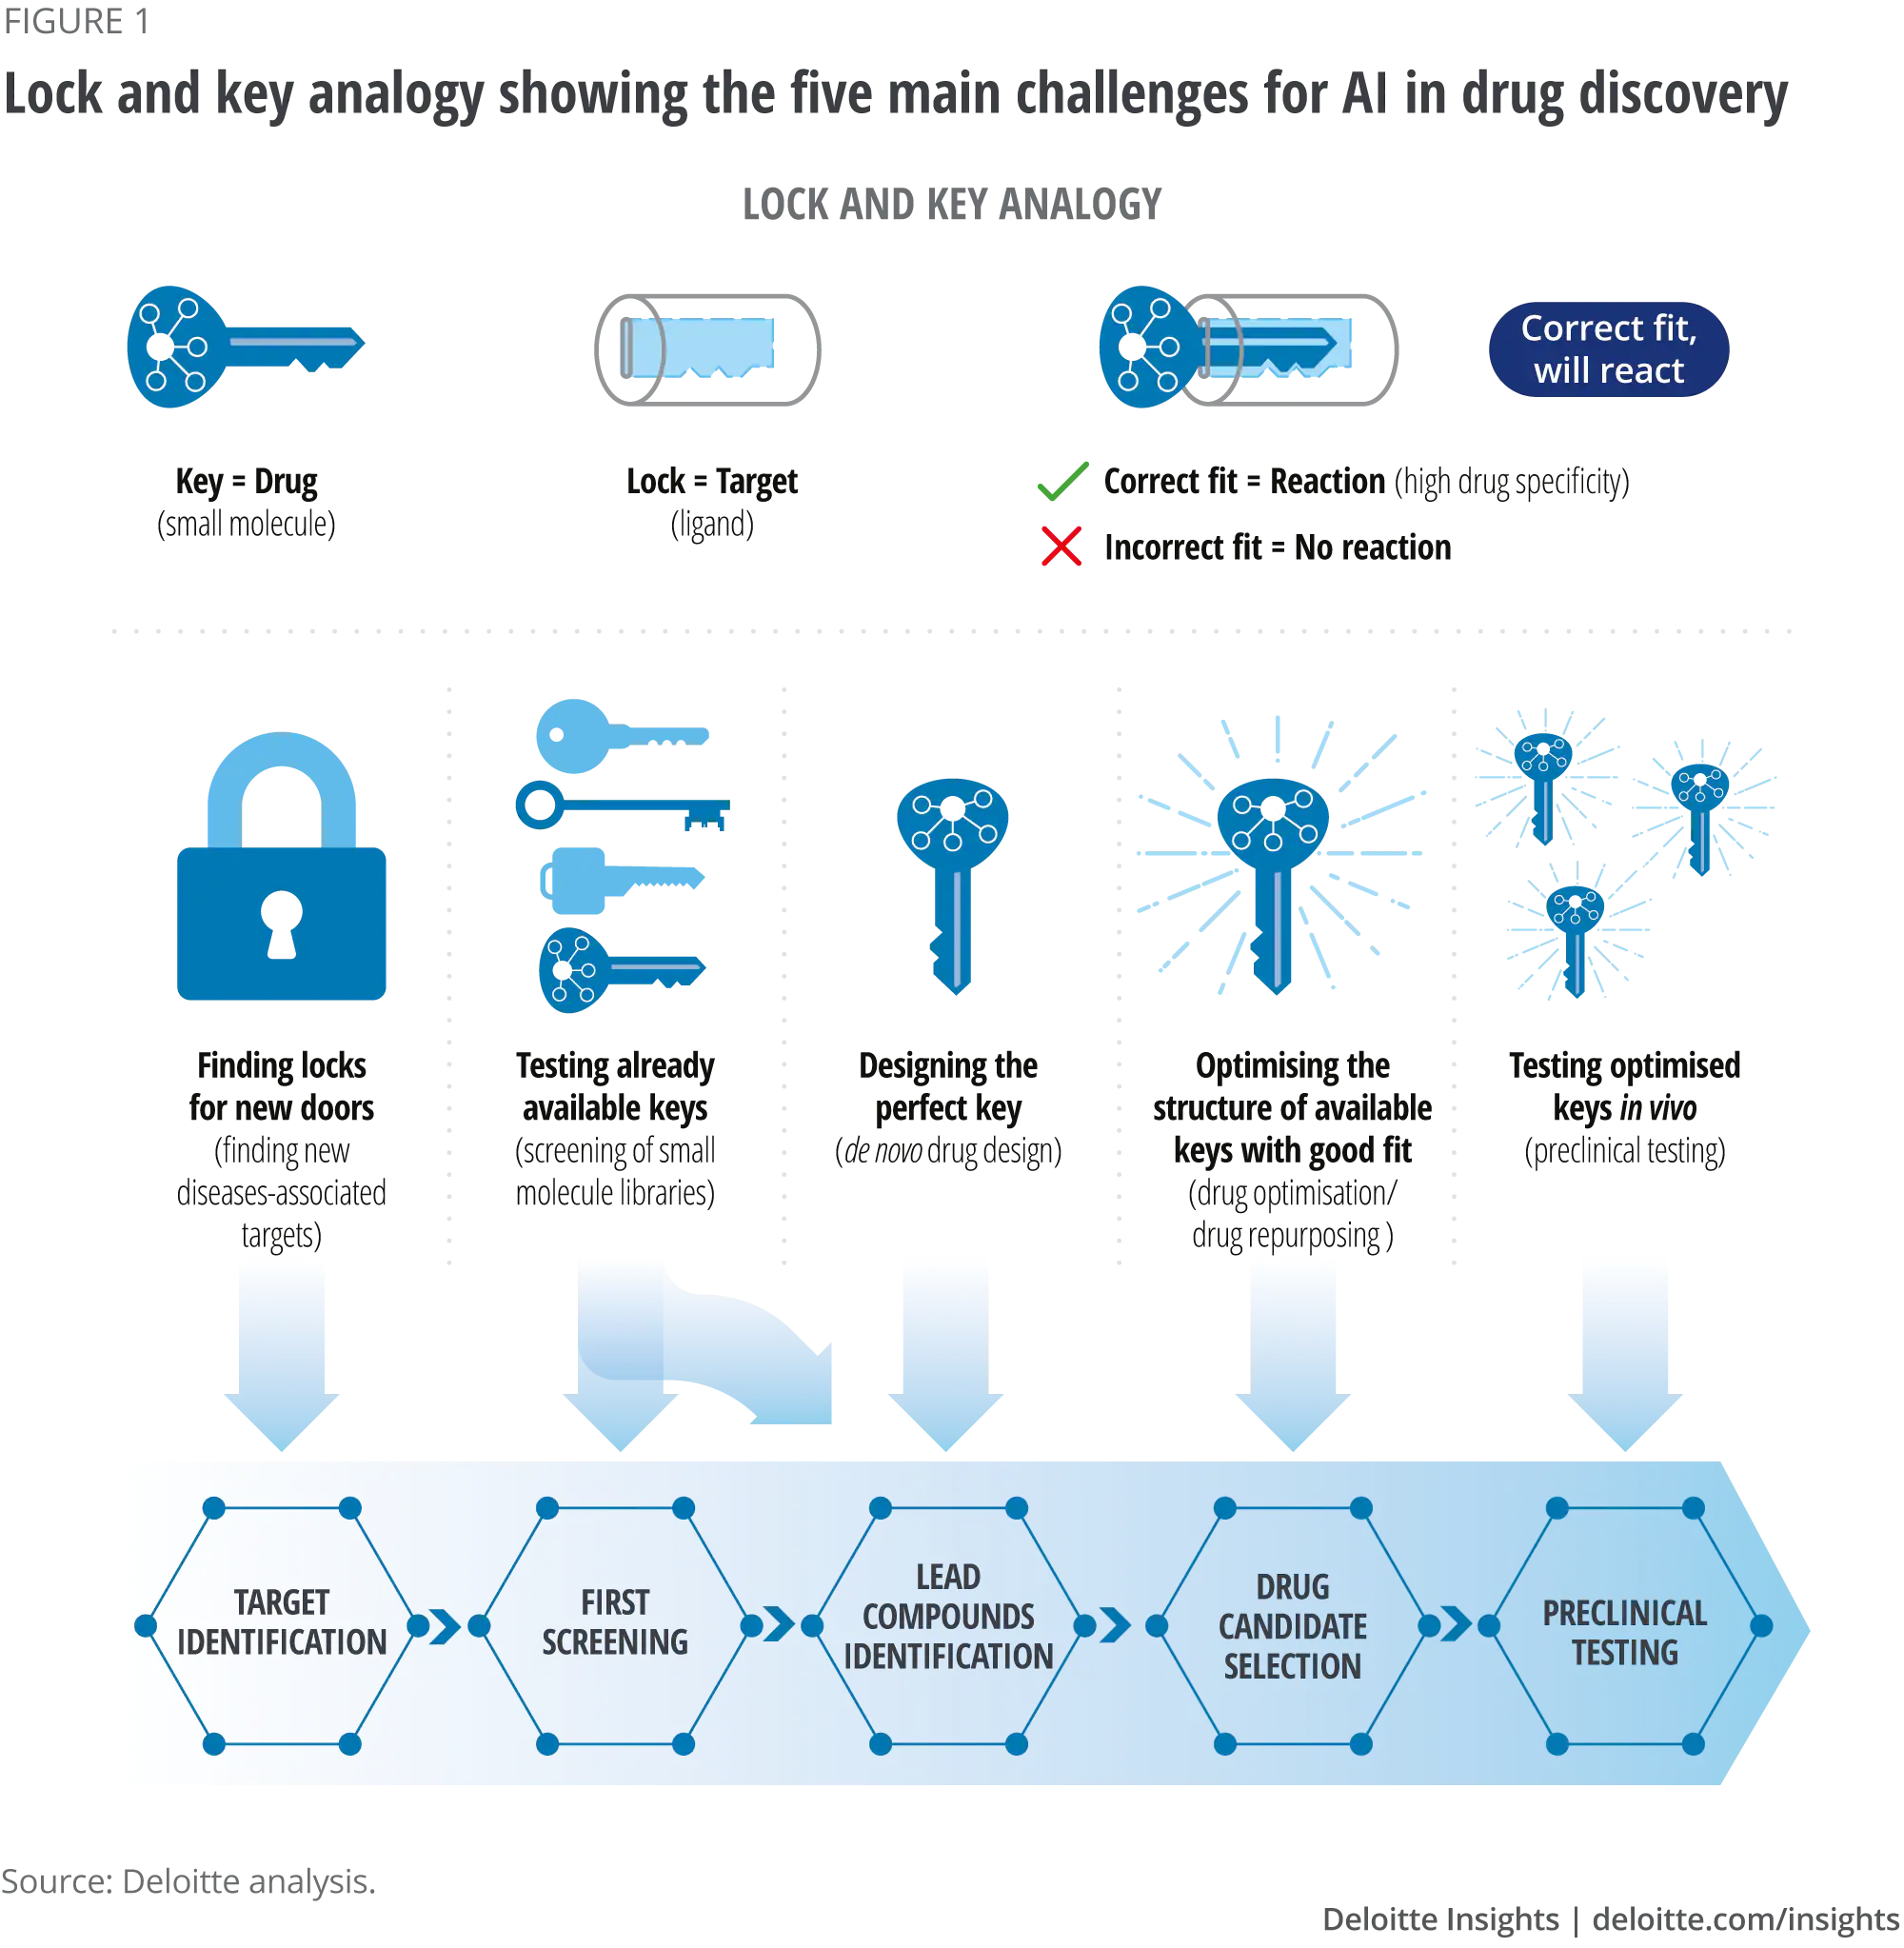
\includegraphics[height=0.8\textheight]{descubrimiento.png}
  \end{figure}
\end{frame}

\begin{frame}{Aplicaciones}{Diagnóstico asistido por computadora}
  En imagenología médica, se utilizan imágenes para analizar al paciente y lograr su diagnóstico. Los sistemas de diagnóstico asistido por computadora aplican la visión computacional para mejorar las capacidades de diagnóstico y mejorar la precisión con el objetivo de salvar vidas.
  \begin{figure}[]
    \centering
    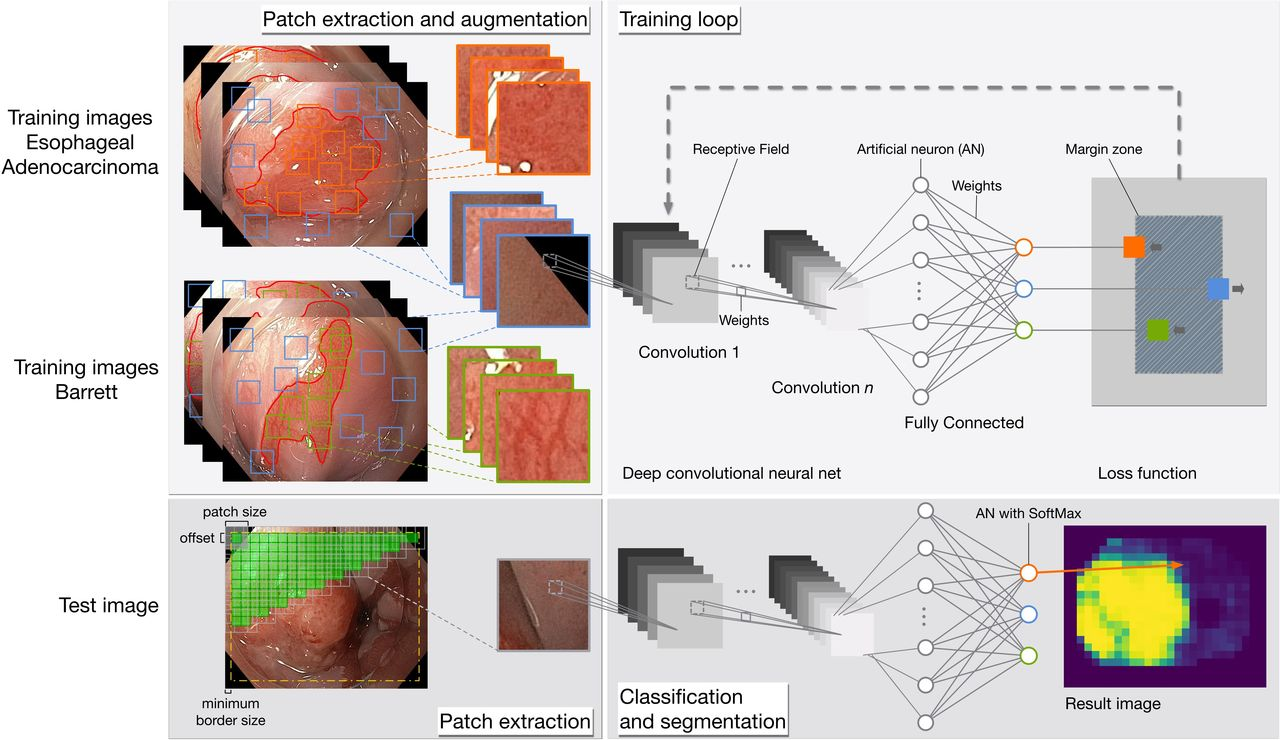
\includegraphics[height=0.70\textheight]{cad.jpg}
  \end{figure}
\end{frame}



\subsection{Cáncer cervicouterino}

\begin{frame}{El Cáncer Cérvicouterino}{Factores y síntomas}
  \begin{figure}[]
    \centering
    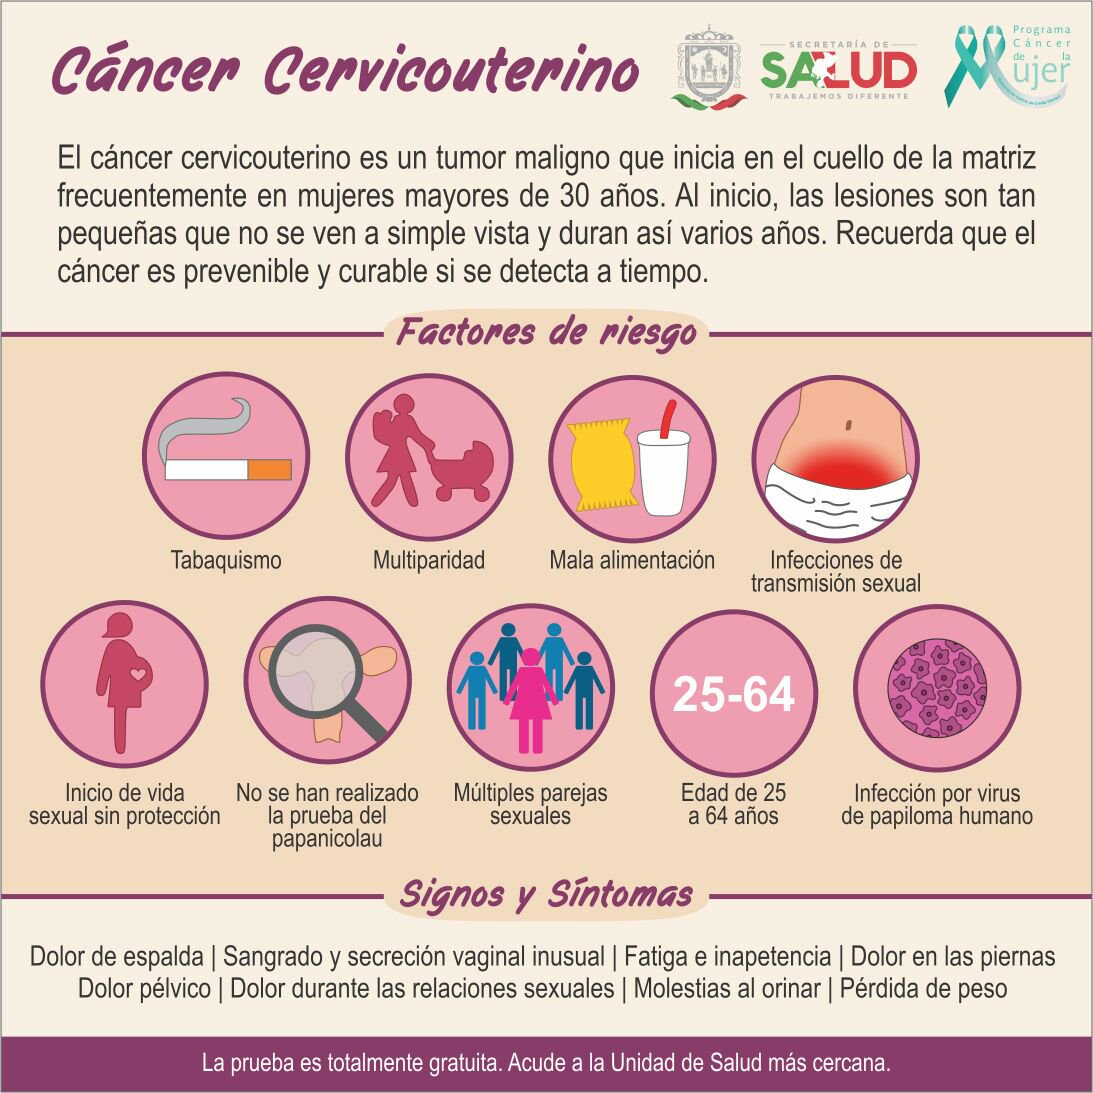
\includegraphics[height=0.95\textheight]{secretaria}
    % \caption{Desarrollo del cáncer}\label{fig:desarrollo}
  \end{figure}
\end{frame}

\begin{frame}{El Cáncer Cérvicouterino}{Datos y estadísticas}
  \begin{block}{Estadísticas}{
      \begin{itemize}
        \item La séptima neoplasia más frecuente a nivel mundial y la cuarta entre mujeres.
        \item 85\% de los casos son en países en vías de desarrollo.
        \item La tendencia de mortalidad es descendente.
        \item Es un indicador de la desigualdad.
        \item Primera causa de muerte por tumor en países en vías de desarrollo.
              % \item El 75\% de las defunciones en LA ocurren en seis países, incluido México.
        \item Segunda muerte por cáncer en la mujer mexicana.
        \item 14000 nuevos casos al año en México.
        \item 10 muertes por día, 4700 al año.
              % \item Se hacen en México 5 millones de pruebas citológicas.
      \end{itemize}
    }
  \end{block}
\end{frame}

\begin{frame}{El problema}{Proceso patológico}

  \begin{block}{Factores de prognosis}
    {
      \begin{itemize}
        \item El cáncer es progresivo.
        \item Es etapas avanzadas, es incurable.
        \item Detección temprana es la primera defensa.
      \end{itemize}
    }
  \end{block}

  \begin{exampleblock}{Factores de diagnóstico}
    {
      \begin{itemize}
        \item Se toma una muestra del paciente
        \item Se usa microscopio para el diagnóstico.
        \item Se realiza un análisis morfológico.
      \end{itemize}
    }
  \end{exampleblock}
\end{frame}

\begin{frame}{El problema}{Condiciones del diagnóstico}

  \begin{alertblock}{Incidencias negativas en la eficacia}{
      \begin{itemize}
        \item Se generan cinco millones de muestras al año.
        \item Poco personal para el diagnóstico.
        \item Error humano en la toma de muestras.
        \item Error humano por fatiga y sobretrabajo.
        \item Deterioro en la visión.
        \item Subjetividad e incertidumbre inherentes al proceso humano.
      \end{itemize}
    }
  \end{alertblock}
\end{frame}

\begin{frame}{Definir el problema}{Detectar y clasificar células cervicales}
  \begin{figure}[]
    \centering
    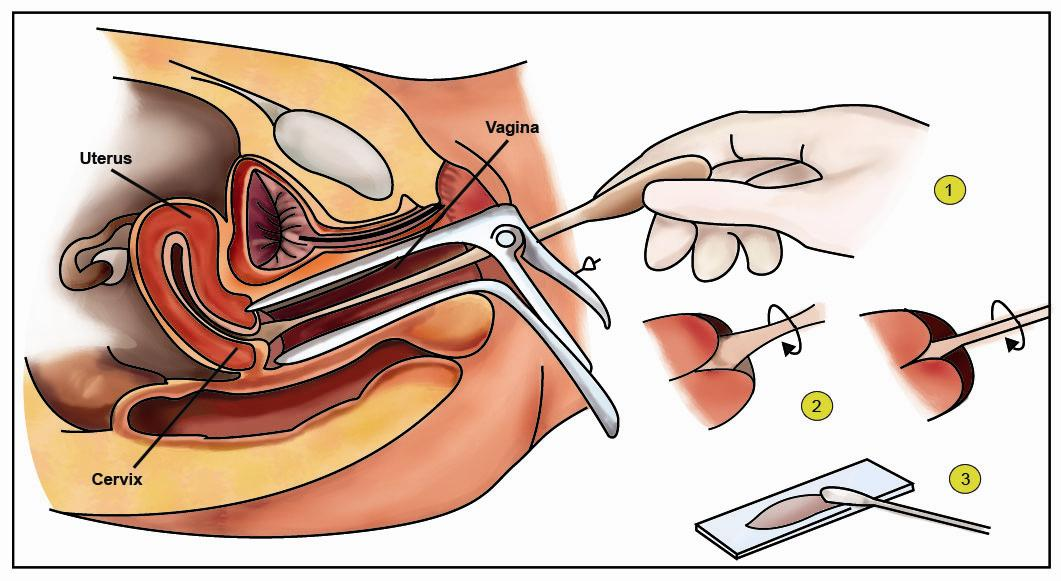
\includegraphics[height=0.95\textheight]{papsmear.jpg}
  \end{figure}
\end{frame}

\begin{frame}{Definir el problema}{Relación entre el daño celular y el cáncer}
  \begin{columns}
    \column{.5\textwidth}
    \begin{exampleblock}{Morfología}
      \begin{itemize}
        \item Existen distintos tipos de células cervicales.
        \item El cáncer comienza con pequeñas lesiones inflamatorias en las células.
        \item Es un proceso progresivo.
        \item Se buscan células atípicas para el diagnóstico.
        \item La detección temprana es crucial.
      \end{itemize}
    \end{exampleblock}
    \column{.5\textwidth}
    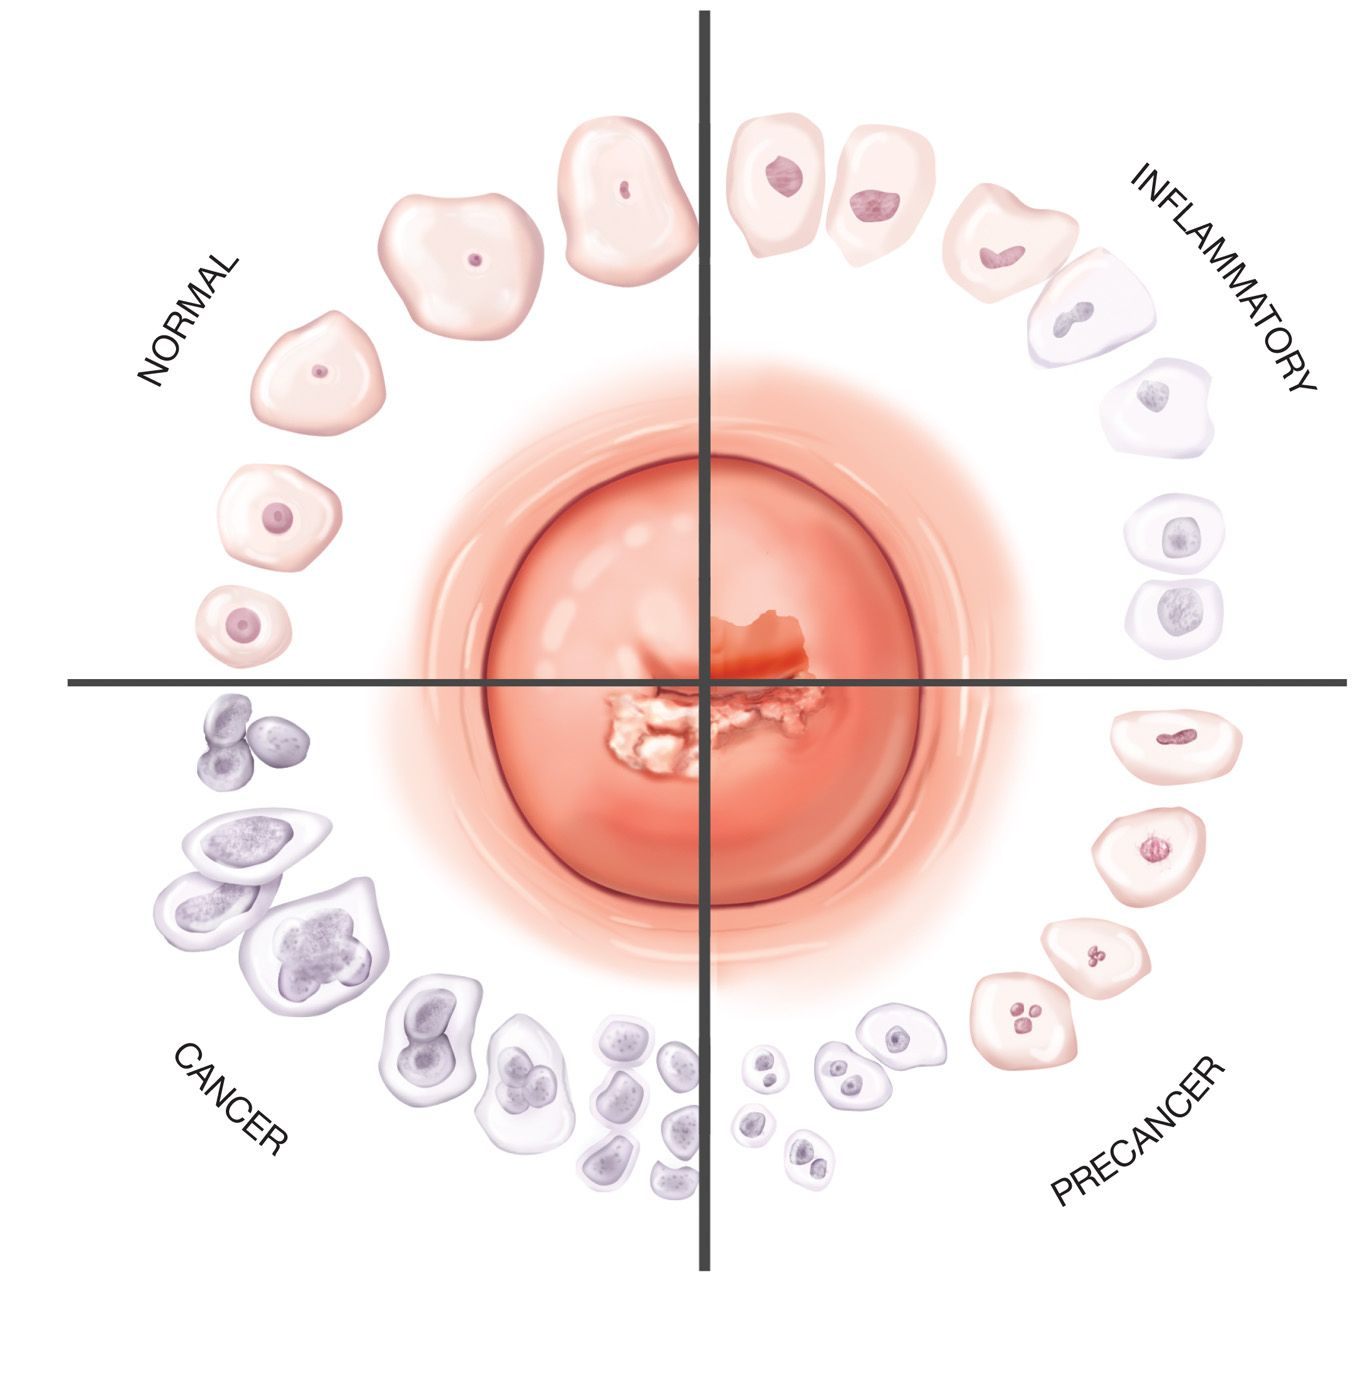
\includegraphics[width=\columnwidth]{ciclo.jpg}
  \end{columns}
\end{frame}

\section{Dependencias teóricas}


% Una vez definida la tarea, delimitamos el problema, es decir, determinar la existencia de celulas atipicas en una prueba de papanicolau analizando imagenes de las celulas individuales.

\subsection{Visión por computadora}

\begin{frame}{Procesamiento digital de imágenes}{Representación de imágenes digitales}
  \begin{columns}
    \column{.5\textwidth}
    \begin{block}{Espacios de color}
      \begin{itemize}
        \item Existen muchos tipos.
        \item El más común es RGB.
        \item Representación matricial de una imagen en tres canales: rojo, verde y azul.
        \item Las imágenes son de la forma $ (pixeles de ancho \times pixeles de alto \times 3) $.
        \item Cada pixel es un vector de tres componentes, donde cada componente tiene un rango $ x \in [0, 255] $.
      \end{itemize}
    \end{block}
    \column{.5\textwidth}
    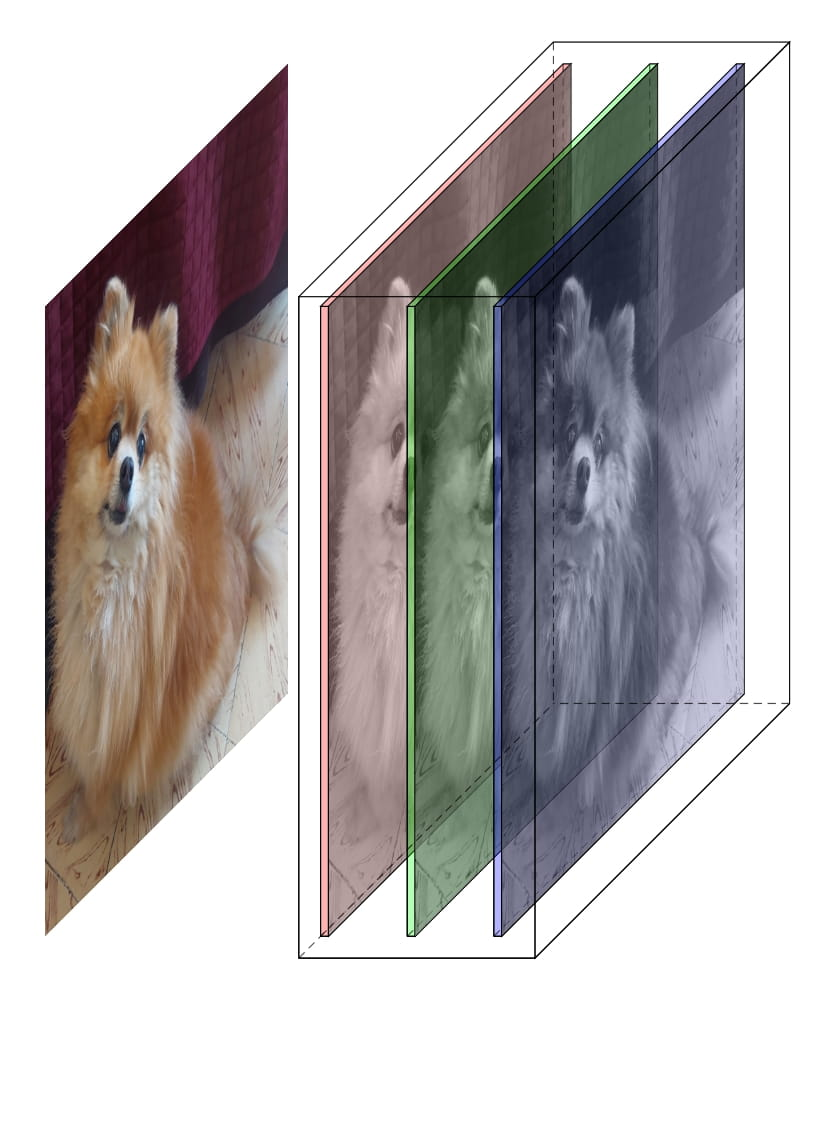
\includegraphics[width=\columnwidth, height=0.9\textheight]{cachito.jpg}
  \end{columns}
\end{frame}


\section{Dependencias tecnológicas}
\subsection{Lenguajes y módulos}

\begin{frame}{Python}{Breve introducción}
  % Desarrollado por Guido Van Rossum el 20 de febrero de 1991. La estructura visual del programa representa de manera precisa su estructura semántica.
  % Al ser muy usado existen bastantes recursos tanto en ingles como en espa;ol
  \begin{columns}
    \column{.5\textwidth}
    \begin{exampleblock}{Características}
      \begin{itemize}
        \item Guido Van Rossum, 20 de febrero de 1991.
        \item Lenguaje interpretado con REPL.
        \item Alto nivel y propósito general.
        \item Multiparadigma: OO, estructurado, funcional.
        \item Fuertemente tipado y evaluación perezosa.
        \item Implementado en C.
        \item Fácil gestión de ambientes y control de módulos.
        \item Estadísticas: \href{https://www.tiobe.com/tiobe-index/}{TIOBE} / \href{https://insights.stackoverflow.com/survey/2021}{StackOverflow}
      \end{itemize}
    \end{exampleblock}
    \column{.5\textwidth}
    
\includegraphics[width=\columnwidth]{python.png}
  \end{columns}
\end{frame}

\begin{frame}{Uso de Python}{Empresas y sistemas}
  % Algunas empresas que san python son Intel, IBM, Nasa, Pixar, Facebook, Google, Reddit
  \begin{columns}
    \column{.3\textwidth}
    
\includegraphics[height=0.4\textheight]{instagram.png}
    \column{.3\textwidth}
    
\includegraphics[height=0.4\textheight]{pinterest.png}
    \column{.3\textwidth}
    
\includegraphics[height=0.4\textheight]{spotify.png}
  \end{columns}

  \begin{table}[]
    \centering
    \begin{tabular}{@{}ccccc@{}}
      
\includegraphics[height=1cm]{intel.png} & 
\includegraphics[height=1.5cm]{nasa.png} & 
\includegraphics[height=1.5cm]{pixar.jpg} & 
\includegraphics[height=1.5cm]{meta.jpg} & 
\includegraphics[height=1.5cm]{google.png}
    \end{tabular}
  \end{table}

\end{frame}

\begin{frame}{Módulos}{Algunos módulos famosos}
  \begin{table}[]
    \centering
    \begin{tabular}{@{}ccccc@{}}
      
\includegraphics[height=1.5cm]{numpy.png} & 
\includegraphics[height=1.5cm]{pandas.png} & 
\includegraphics[height=1.5cm]{matplotlib.png} & 
\includegraphics[height=1.5cm]{tensorflow.png} & 
\includegraphics[height=1.5cm]{scikit.png} \\
      Matemáticas                               & Datos tabulares                            & Gráficos y figuras                             & I.A.                                           & Machine learning
    \end{tabular}
  \end{table}


  \begin{table}[]
    \centering
    \begin{tabular}{@{}ccc@{}}
      
\includegraphics[height=1cm]{django.png} & 
\includegraphics[height=1cm]{pillow.png} & 
\includegraphics[height=1.5cm]{jupyter.png} \\
      Web                                      & Imágenes                                 & Cómputo interactivo
    \end{tabular}
  \end{table}

\end{frame}


\end{document}

